% Beamer slide deck for Mathematical Physics
% "Mathematical Physics"
% Chapter 4: Sturm--Liouville Theory
% Self-contained slide text; local figures live in figs.

\documentclass[11pt]{beamer}

\usepackage[utf8]{inputenc}
\usepackage[T1]{fontenc}
\usepackage{lmodern}
\usepackage{amsmath,amssymb}
\usepackage{graphicx}
\usepackage{tikz}

\usetheme{Madrid}

\author[]{Compiled by Jake W. Liu}
\title[Sturm--Liouville Theory]{Chapter 4: Sturm--Liouville Theory}
\subtitle{Mathematical Physics}
\date{\today}

\setbeamertemplate{navigation symbols}{}
\setbeamertemplate{frametitle continuation}[from second]

% Per-section TOC frames removed to keep the deck within 60 slides.

\usepackage{Kyushu}

% Neutralize \index so source markup (if any) is harmless.
\makeatletter
\@ifundefined{index}{\newcommand{\index}[1]{}}{\renewcommand{\index}[1]{}}
\makeatother

\begin{document}

% Forest-first revision: classical calculus + formal adjoints via IBP.
% Domain = sufficiently smooth functions with BCs that kill the boundary form.
% No Sobolev/Hilbert jargon; intermediate algebra kept explicit.

\newcounter{sfchapter}
\setcounter{sfchapter}{4}
\renewcommand{\thesection}{\arabic{sfchapter}.\arabic{section}}
\numberwithin{equation}{section}

\begin{frame}[c]\titlepage
\end{frame}

\begin{frame}{Outline}
\tableofcontents
\end{frame}

\begin{frame}{Where we are going}
\footnotesize
\textbf{Why.} Separating variables in the wave, heat and Laplace equations (a
vibrating string, a drum, a heated rod) leaves an ODE eigenvalue problem for the
spatial \emph{modes}. We want one theory that says why these modes are orthogonal
and how to expand any initial shape in them. It needs only calculus and inner
products of functions.
\begin{itemize}
  \item Functions act as vectors; Fourier coefficients are extracted by orthogonality.
  \item The Sturm--Liouville eigenvalue problem, with this chapter's sign convention, is
        \[
          \frac{d}{dx}\left(p(x)\frac{du}{dx}\right)+q(x)u(x)
          =-\lambda w(x)u(x),
        \]
        typically with $p>0$ and $w>0$ inside the interval. For a string, $p$ is the
        tension, $w$ the mass per length, and $\lambda=\omega^2$ the squared angular
        frequency of the mode.
  \item Integration by parts gives the \emph{formal adjoint}; boundary conditions that
        kill the boundary term make the problem symmetric, like a symmetric matrix.
  \item Symmetry then yields real eigenvalues and orthogonal eigenfunctions.
  \item Legendre and Bessel (drum) modes illustrate the theory, and an integrating
        factor brings any real second-order equation into this form (where its
        leading coefficient is nonzero).
  \item A point source then defines the Green function.
\end{itemize}
\end{frame}

% ======================================================================
\section{Review of linear algebra}
% ======================================================================

\begin{frame}[allowframebreaks=1.00]{Vector spaces and bases}
\footnotesize

A \emph{vector space} is a collection of objects that is closed under addition and
scalar multiplication: if $u$ and $v$ belong to the space and $a,b$ are scalars,
then $au+bv$ also belongs to the space.  The vectors may be functions rather than
geometric arrows.

\medskip
\textbf{Examples.}
\begin{itemize}
  \item The polynomials of degree at most two,
        $a_0+a_1x+a_2x^2$, form a three-dimensional vector space.
  \item The smooth functions on $[0,1]$ satisfying $u(0)=u(1)=0$ form a vector
        space, because
        \[
          (au+bv)(0)=au(0)+bv(0)=0,
          \qquad
          (au+bv)(1)=au(1)+bv(1)=0.
        \]
\end{itemize}

A \emph{basis} is a set of vectors from which every vector in the space has a
unique linear combination. Existence is called \emph{spanning}; uniqueness follows
from \emph{linear independence} (only zero coefficients give the zero vector).
For the quadratic
polynomials, $\{1,x,x^2\}$ is a basis, and
\begin{equation}
  1+2x+3x^2=1\cdot1+2\cdot x+3\cdot x^2.
  \label{eq:basis-mono}
\end{equation}

The number of elements in a finite basis is the \emph{dimension}.  Mode expansions
use infinitely many basis functions, so we first need a way to measure length and
angle between functions (an inner product), and then convergence.
\end{frame}

\begin{frame}[allowframebreaks=1.00]{Inner products, norms, and coefficients}
\footnotesize

\textbf{Goal.} Expand a function in a set of ``mode'' functions, \(f=\sum a_iu_i\), and find the coefficients
\(a_i\). For ordinary vectors we would use the dot product; we need the same tool for functions.

\textbf{Step 1: from dot product to integral.} For vectors in \(\mathbb R^N\),
\(u\cdot v=\sum_{k}u_kv_k\). Think of a function \(u(x)\) on \([a,b]\) as a vector with very many
components: its values \(u(x_k)\) at closely spaced points \(x_k\), spacing \(\Delta x\). Then
\(\sum_ku(x_k)v(x_k)\,\Delta x\to\int_a^bu(x)v(x)\,dx\). So the natural ``dot product'' of functions is an
integral. For complex-valued functions we also conjugate the second factor (reason below):
\begin{equation}
  (u,v)=\int_a^b u(x)\overline{v(x)}\,dx.
  \label{eq:l2ip}
\end{equation}
\textbf{The rules.} An inner product \((\cdot,\cdot)\) must satisfy (we take it linear in the first slot):
\begin{enumerate}
  \item \((au+bv,w)=a(u,w)+b(v,w)\); in particular \((cu,v)=c\,(u,v)\) for a number \(c\);
  \item \((u,v)=\overline{(v,u)}\);
  \item \((u,u)\geq0\), with equality only for \(u=0\).
\end{enumerate}
\par\framebreak\par
\textbf{Why the conjugate?} Without it, \((u,u)=\int u^2dx\) could be negative or complex for complex \(u\)
(try \(u=i\)), and could not be a squared length. With it, \((u,u)=\int|u|^2dx\ge0\).

\textbf{A consequence: the second slot is conjugate-linear.} Swap the slots (rule~2), pull out \(c\)
(rule~1), and swap back:
\begin{equation}
  (u,cv)=\overline{(cv,u)}=\overline{c\,(v,u)}
  =\overline{c}\;\overline{(v,u)}=\overline{c}\,(u,v).
  \label{eq:ip-conj-linear-second}
\end{equation}
\textbf{Weighted inner product.} Sometimes different points should count differently. With a real
weight \(w(x)>0\) inside \((a,b)\) (it may vanish at an endpoint),
\begin{equation}
  (u,v)_w=\int_a^b u(x)\overline{v(x)}\,w(x)\,dx.
  \label{eq:wip}
\end{equation}
For example, on a disk (the drum problem later in this chapter) a ring at radius $s$
has area $2\pi s\,ds$, so the weight $w(s)=s$ counts each radius by its area.

\textbf{Length and angle.} The length (norm) is
\begin{equation}
  \|u\|=\sqrt{(u,u)},
  \qquad
  \|u\|_w=\sqrt{(u,u)_w},
  \label{eq:induced-norm}
\end{equation}
and $u/\|u\|$ has length one.  Two vectors are \emph{orthogonal} when $(u,v)=0$;
an \emph{orthonormal} set satisfies $(u_i,u_j)=\delta_{ij}$, where $\delta_{ij}=1$ for $i=j$ and $0$ otherwise.

\par\framebreak\par
\textbf{Step 2: extract coefficients by orthogonality.}  Suppose
$f=\sum_{i=1}^{N}a_iu_i$ with orthogonal $u_i$.  Take the inner product with $u_j$;
by linearity in the first slot, and because $(u_i,u_j)=0$ for $i\ne j$, only the
$i=j$ term survives:
\[
  (f,u_j)=\sum_{i=1}^{N}a_i(u_i,u_j)=a_j(u_j,u_j)=a_j\|u_j\|^2.
\]
So
\begin{equation}
  a_j=\frac{(f,u_j)}{\|u_j\|^2},
  \label{eq:coeff-orthogonal}
\end{equation}
which is simply $a_j=(f,u_j)$ for an orthonormal set.  Geometrically, $a_ju_j$ is the
projection of $f$ onto the $u_j$ direction, just as $f\cdot e_x$ picks the
$x$-component of a vector in $\mathbb R^3$.  The same formula serves infinite
sums (next frame).
\end{frame}

\begin{frame}[allowframebreaks=1.00]{Infinite-dimensional bases and $L^2$}
\footnotesize
\textbf{The new issue.} Mode expansions use infinitely many functions, so they are infinite series. We
must say in what sense the partial sums approach \(f\).

\textbf{Distance between functions.} Use the length from \eqref{eq:induced-norm} on \([0,1]\):
\[
 \|f\|_2=\left(\int_0^1|f(x)|^2\,dx\right)^{1/2},\qquad \text{distance}(f,g)=\|f-g\|_2 .
\]
The functions with \(\|f\|_2<\infty\) form the space \(L^2(0,1)\).

\textbf{Orthogonal is not enough; we also need complete.} Take the sine modes \(u_n(x)=\sin(n\pi x)\),
\(n=1,2,\ldots\) (the next frame shows that they are orthogonal, with \(\|u_n\|^2=\frac12\)). Suppose we threw
away \(u_1\). The remaining modes could not rebuild it: every coefficient \((u_1,u_n)/\|u_n\|^2\) with \(n\ge2\) is
zero, so the expansion of \(u_1\) would be \(0\). (Like trying to build the \(z\)-axis out of the \(x\)- and
\(y\)-axes.) A set of modes that misses no direction is called \emph{complete}.
\par\framebreak\par
\textbf{The sine modes are complete} (quoted from Fourier analysis). Every \(f\) in \(L^2(0,1)\) can be
expanded as
\[
 f=\sum_{n=1}^{\infty}a_nu_n,\qquad
 a_n=\frac{(f,u_n)}{\|u_n\|^2},
\]
which is the projection formula \eqref{eq:coeff-orthogonal} with infinitely many terms.

\textbf{In what sense?} In the \emph{mean-square} sense: the distance between \(f\) and the partial sum
goes to zero,
\[
 \Bigl\|f-\sum_{n=1}^{N}a_nu_n\Bigr\|_2\longrightarrow0\qquad(N\to\infty).
\]
This controls the total squared error, not the error at every single point. The example \(f=1\) below
shows the difference: the partial sums stay \(0\) at the endpoints, yet the total error shrinks.
\end{frame}

\begin{frame}[allowframebreaks=1.00]{Example: orthogonality of the sine modes}
\footnotesize
Let $u_m(x)=\sin(m\pi x)$ and $u_n(x)=\sin(n\pi x)$, with $m,n$ positive integers.
Use the product-to-sum identity
\begin{equation}
 \sin A\sin B=\tfrac12[\cos(A-B)-\cos(A+B)].\label{eq:sinsin}
\end{equation}
For $m\ne n$, apply \eqref{eq:sinsin} with $A=m\pi x$, $B=n\pi x$ and integrate
each cosine term:
\begin{align}
 \int_0^1u_mu_n\,dx
 &=\frac12\int_0^1\bigl[\cos((m-n)\pi x)-\cos((m+n)\pi x)\bigr]dx\notag\\
 &=\left[\frac{\sin((m-n)\pi x)}{2(m-n)\pi}
        -\frac{\sin((m+n)\pi x)}{2(m+n)\pi}\right]_0^1\notag\\
 &=0,\label{eq:sin-mn}
\end{align}
because sine is zero at every integer multiple of $\pi$.
For $m=n$, use $\sin^2(m\pi x)=[1-\cos(2m\pi x)]/2$, which is \eqref{eq:sinsin} with $A=B=m\pi x$ and $\cos 0=1$:
\begin{equation}
 \int_0^1u_m^2\,dx
 =\left[\frac{x}{2}-\frac{\sin(2m\pi x)}{4m\pi}\right]_0^1
 =\frac12.\label{eq:sin-nn}
\end{equation}
Together,
\begin{equation}
 (u_m,u_n)=\tfrac12\delta_{mn},\label{eq:sin-orth}
\end{equation}
so the functions $\sqrt2\,u_n$ are orthonormal.
\end{frame}

\begin{frame}{Example: Fourier sine-series coefficients}
\footnotesize
For $f\in L^2(0,1)$, write $f(x)=\sum_{n=1}^{\infty}a_n\sin(n\pi x)$ in the
mean-square sense.  The projection formula \eqref{eq:coeff-orthogonal} and the norm
$\|u_n\|^2=1/2$ from \eqref{eq:sin-nn} give
\begin{equation}
 a_n=\frac{(f,u_n)}{\|u_n\|^2}
 =\frac{\int_0^1 f(x)\sin(n\pi x)\,dx}{1/2}
 =2\int_0^1 f(x)\sin(n\pi x)\,dx.\label{eq:sine-transform}
\end{equation}
The factor $2$ comes from the norm $1/2$, not from an extra convention.

\begin{columns}[T]
\begin{column}{0.53\textwidth}
\textbf{Example: $f(x)=1$.} By \eqref{eq:sine-transform},
$a_n=2\bigl[-\cos(n\pi x)/(n\pi)\bigr]_0^1=2\bigl(1-(-1)^n\bigr)/(n\pi)$,
i.e.\ $a_n=4/(n\pi)$ for odd $n$ and $0$ for even $n$.  In the plot, the partial
sums stay $0$ at $x=0,1$ and overshoot near the ends (the peak stays near $1.18$ as
$N$ grows), yet the band
where they differ from $1$ narrows, so the error norm
$\|f-\sum_{n\le N}a_nu_n\|_2$ falls from $0.32$ ($N=3$) to $0.14$ ($N=21$).
That is mean-square convergence.
\end{column}
\begin{column}{0.45\textwidth}
\begin{tikzpicture}[x=3.8cm,y=1.9cm]
 \draw[->] (0,0) -- (1.06,0) node[right] {$x$};
 \draw[->] (0,0) -- (0,1.38);
 \foreach \t in {0.5,1} \draw (0.01,\t) -- (-0.01,\t) node[left] {$\t$};
 \draw (1,0.02) -- (1,-0.02) node[below] {$1$};
 \draw[dashed,gray] (0,1) -- (1,1);
 \draw[blue!70!black,thick] plot[domain=0:1,samples=121,smooth]
   (\x,{4/pi*(sin(180*\x)+sin(540*\x)/3)});
 \draw[red!75!black] plot[domain=0:1,samples=301]
   (\x,{4/pi*(sin(180*\x)+sin(540*\x)/3+sin(900*\x)/5+sin(1260*\x)/7+sin(1620*\x)/9+sin(1980*\x)/11+sin(2340*\x)/13+sin(2700*\x)/15+sin(3060*\x)/17+sin(3420*\x)/19+sin(3780*\x)/21)});
 \node[blue!70!black,anchor=north] at (0.5,0.62) {$N=3$};
 \node[red!75!black,anchor=south] at (0.5,1.2) {$N=21$};
\end{tikzpicture}
\end{column}
\end{columns}

\smallskip
The same projection rule will give coefficients for Bessel and polynomial expansions;
only the interval, weight, and norm will change.
\end{frame}

\begin{frame}[allowframebreaks=1.00]{Linear operators and formal adjoints}
\footnotesize

\textbf{Goal.} Eigenvalues of a symmetric matrix are real and its eigenvectors are orthogonal.
We want the same for differential operators, so we must find out which of them behave like
symmetric matrices. The test is integration by parts.

\textbf{A linear operator acts on functions.} It satisfies
$L(au+bv)=aLu+bLv$. Differentiation, multiplication by a fixed function, and
$Au(x)=\int_{x_0}^{x}u(t)\,dt$ are examples.
The allowed functions must also satisfy any specified boundary conditions.

\textbf{Matrix picture.} For a matrix, $(u,Av)=(A^\dagger u,v)$ with
$A^\dagger=\overline{A}^{T}$, and $A$ is symmetric (Hermitian) when $A^\dagger=A$.
For a differential operator, integration by parts plays the role of transposing.

\textbf{Integration by parts moves a derivative.} Recall \(\int_0^1fg'\,dx=[fg]_0^1-\int_0^1f'g\,dx\). Use it
with \(f=u\), \(g=\overline v\), for the operator \(D=d/dx\):
\begin{equation}
 (u,Dv)=\int_0^1u\overline{v'}\,dx
 =\left[u\overline v\right]_0^1-\int_0^1u'\overline v\,dx
 =\left[u\overline v\right]_0^1+(-Du,v).
 \label{eq:ddx-adjoint-general}
\end{equation}
So moving \(D\) from \(v\) to \(u\) costs a minus sign, plus a boundary term. The operator that appears on
\(u\) (ignoring the boundary term) is called the \emph{formal adjoint}: here \(D^\dagger=-D\). So \(D\) behaves
like an antisymmetric matrix (\(A^T=-A\)), not a symmetric one.

\textbf{Two derivatives: two minus signs cancel,} as \((-D)(-D)=D^2\) suggests. For \(L=D^2\), integrate by
parts once (first line), then once more on \(\int u'\overline{v'}\) (second line):
\begin{align}
 (u,Lv)&=\int_0^1u\overline{v''}\,dx\notag\\
 &=\left[u\overline{v'}\right]_0^1-\int_0^1u'\overline{v'}\,dx
 \label{eq:d2-ibp-once}\\
 &=\left[u\overline{v'}-u'\overline v\right]_0^1
   +\int_0^1u''\overline v\,dx.
 \label{eq:d2-ibp-twice}
\end{align}
The operator on \(u\) is again \(D^2\): \(L^\dagger=L\) (``formally self-adjoint''). If moreover the boundary term
vanishes, \(L\) behaves exactly like a symmetric matrix. For example, with \(u(0)=u(1)=v(0)=v(1)=0\)
(Dirichlet conditions) every term of the bracket is zero:
\begin{equation}
 (u,Lv)=(Lu,v).
 \label{eq:d2-adjoint}
\end{equation}
Neumann conditions ($u'=v'=0$ at the ends) kill the bracket too; other boundary
conditions are checked in the next section.  This
symmetry is what makes eigenfunctions with different eigenvalues orthogonal.
\end{frame}

\begin{frame}[allowframebreaks=1.00]{Eigenfunctions and the orthogonality theorem}
\footnotesize
\textbf{Goal.} Show that an operator which is ``symmetric'' in the sense of the previous frame has real
eigenvalues and orthogonal eigenfunctions, exactly as a symmetric matrix does.

An eigenpair $(u,\lambda)$ of an operator $L$ satisfies $Lu=\lambda u$ with
$u\neq0$.  A generalized eigenvalue problem introduces a prescribed real weight
$w(x)$: $Lu=\lambda wu$.  The Sturm--Liouville form of \S\ref{sec:sturm-liouville} puts $-\lambda wu$ on the
right instead; the minus sign makes $\lambda$ positive for the string below
($\lambda=(n\pi)^2$, a squared frequency).

\textbf{Examples.} $(e^{\lambda x})'=\lambda e^{\lambda x}$; and for real $m\neq0$,
$\cos(mx)$ and $\sin(mx)$ are eigenfunctions of $d^2/dx^2$ with eigenvalue $-m^2$.

\textbf{Matrix analogy.} A Hermitian (e.g.\ real symmetric) matrix has real
eigenvalues and orthogonal eigenvectors; the same proof works under the symmetry
\eqref{eq:d2-adjoint}:

\begin{theorem}
Every eigenvalue of a self-adjoint operator (one with $(Lu,v)=(u,Lv)$ for all allowed $u,v$) is real.  Eigenfunctions belonging to
distinct eigenvalues are orthogonal.
\end{theorem}

\textbf{Proof.} Let \(Lu_i=\lambda_i u_i\) and \(Lu_j=\lambda_j u_j\). Compute \((Lu_i,u_j)\) in two ways:
\[
  \underbrace{\lambda_i(u_i,u_j)=(Lu_i,u_j)}_{\text{rule 1}}
  \;\overset{\text{self-adjoint}}{=}\;(u_i,Lu_j)=(u_i,\lambda_j u_j)
  \;\overset{\eqref{eq:ip-conj-linear-second}}{=}\;\overline{\lambda_j}\,(u_i,u_j).
\]
Bring everything to one side: \((\lambda_i-\overline{\lambda_j})\,(u_i,u_j)=0\). Now read this twice.
\begin{itemize}
  \item \emph{Take \(j=i\).} Then \((u_i,u_i)=\|u_i\|^2>0\), so \(\lambda_i-\overline{\lambda_i}=0\): \(\lambda_i\) equals its
        conjugate, so it is real. This holds for every eigenvalue.
  \item \emph{Take \(\lambda_i\ne\lambda_j\).} Since \(\lambda_j\) is real, \(\lambda_i-\overline{\lambda_j}=\lambda_i-\lambda_j\ne0\), so
        \((u_i,u_j)=0\): the eigenfunctions are orthogonal.
\end{itemize}
Section~\ref{sec:sturm-liouville} reuses this argument with a weight \(w\).

For a repeated eigenvalue, orthogonal eigenfunctions can still be chosen
(Gram--Schmidt: subtract from the second its projection \eqref{eq:coeff-orthogonal}
on the first).



\textbf{Application: the fixed string.} Let \(Lu=u''\) on \([0,1]\) with \(u(0)=u(1)=0\).

\emph{Step 1: every eigenvalue is negative.} Let \(Lu=\mu u\) with \(u\neq0\). Take the inner product with \(u\)
and integrate by parts; the boundary term vanishes because \(u(0)=u(1)=0\):
\begin{align*}
  \mu\|u\|^2
   =(Lu,u)
   =\int_0^1u''\overline u\,dx
   =\left[u'\overline u\right]_0^1-\int_0^1|u'|^2\,dx
   =-\int_0^1|u'|^2\,dx<0.
\end{align*}
(Strict, since $u'\equiv0$ would make $u$ constant, hence $0$.)  Physically,
$\int|u'|^2dx$ is the string's stretching energy: any deflection costs energy, so
the squared frequencies $-\mu$ (the $\lambda$ of the Sturm--Liouville form) are positive.

\emph{Step 2: solve.} Write \(\mu=-k^2\) with \(k>0\). Then \(u''+k^2u=0\), so
\(u(x)=A\cos(kx)+B\sin(kx)\). The left end gives \(u(0)=A=0\). The right end gives \(u(1)=B\sin k=0\). A
nonzero eigenfunction needs \(B\neq0\), so \(\sin k=0\), that is, \(k=n\pi\) with \(n=1,2,3,\ldots\). Thus
\begin{equation}
  u_n(x)=\sin(n\pi x),
  \qquad
  Lu_n=-(n\pi)^2u_n.
  \label{eq:string-eigenpairs}
\end{equation}
By \eqref{eq:d2-adjoint} $L$ is self-adjoint here, so the theorem gives
$(u_m,u_n)=0$ for $m\neq n$, as the direct integral \eqref{eq:sin-orth} found.
\end{frame}

% ======================================================================
\section{Sturm--Liouville operators}
\label{sec:sturm-liouville}
% ======================================================================

\begin{frame}[allowframebreaks=1.00]{Formal adjoint of a second-order expression}
\footnotesize
\textbf{Goal.} $D^2$ was self-adjoint and gave orthogonal sine modes. Which
second-order expressions share this property? With real coefficients, write
\begin{equation}
 \ell[u]=p_0u''+p_1u'+p_2u.\label{eq:Lgen}
\end{equation}
\textbf{Step 1: move all derivatives from \(u\) to \(v\).} Integrate the \(u''\) term by parts twice (each time the
derivative leaves \(u\) and lands on the factor \(p_0\overline v\)), and the \(u'\) term once:
\begin{align*}
 \int_a^b p_0u''\overline v\,dx
  &=\left[p_0u'\overline v\right]_a^b-\int_a^b u'(p_0\overline v)'\,dx\\
  &=\left[p_0u'\overline v-u(p_0\overline v)'\right]_a^b
    +\int_a^b u(p_0\overline v)''\,dx,\\
 \int_a^b p_1u'\overline v\,dx
  &=\left[p_1u\overline v\right]_a^b-\int_a^b u(p_1\overline v)'\,dx.
\end{align*}
\textbf{Step 2: collect.} Add the untouched term \(\int_a^b p_2u\overline v\,dx\). In the inner product \eqref{eq:l2ip},
\begin{equation}
 (\ell[u],v)
  =\bigl[\text{boundary terms}\bigr]_a^b
  +\int_a^b u\left[(p_0\overline v)''-(p_1\overline v)'+p_2\overline v\right]dx.
 \label{eq:formal-adjoint-ibp}
\end{equation}
Because the coefficients are real, the last integrand is
$u\,\overline{(p_0v)''-(p_1v)'+p_2v}$, so the integral is $(u,\ell^\dagger[v])$ with
the formal adjoint
\begin{equation}
 \ell^\dagger[v]=(p_0v)''-(p_1v)'+p_2v.\label{eq:Lstar}
\end{equation}
\textbf{Step 3: when is \(\ell^\dagger=\ell\)?} Expand by the product rule,
\((p_0v)''=p_0v''+2p_0'v'+p_0''v\) and \((p_1v)'=p_1v'+p_1'v\):
\[
 \ell^\dagger[v]=p_0v''+(2p_0'-p_1)\,v'+(p_0''-p_1'+p_2)\,v .
\]
Compare with \(\ell[v]=p_0v''+p_1v'+p_2v\), coefficient by coefficient:
\begin{itemize}
  \item \(v''\): \(p_0=p_0\). Always true.
  \item \(v'\): \(2p_0'-p_1=p_1\), that is, \(p_1=p_0'\).
  \item \(v\): \(p_0''-p_1'+p_2=p_2\), that is, \(p_1'=p_0''\). This follows from the previous line by
        differentiating.
\end{itemize}
Hence
\begin{equation}
 \ell^\dagger=\ell\quad\Longleftrightarrow\quad p_1=p_0'.\label{eq:pp1}
\end{equation}
\textbf{Message.} \(p_1=p_0'\) means \(p_0u''+p_1u'=(p_0u')'\) (product rule). So a second-order expression is
formally self-adjoint exactly when its derivative terms combine into \((p_0u')'\). The boundary term in
\eqref{eq:formal-adjoint-ibp} must still vanish on the allowed functions; the next frame computes it in a
cleaner form.
\end{frame}

\begin{frame}[allowframebreaks=1.00]{The Sturm--Liouville expression and Green's identity}
\footnotesize

\textbf{Goal.} The previous frame left an unevaluated boundary term and the condition $p_1=p_0'$
for formal self-adjointness. Here we rewrite such an expression in its standard compact form and
find the boundary term exactly, as a formula called Green's identity; the eigenvalue theorem
needs it.

\textbf{Step 1: put the expression in divergence form.}  When $p_1=p_0'$ (the self-adjointness condition \eqref{eq:pp1}), the first two terms in \eqref{eq:Lgen} combine by the product rule:
\begin{align*}
  (p_0u')'
   &=p_0'u'+p_0u''\\
   &=p_1u'+p_0u''.
\end{align*}
Writing $p=p_0$ and $q=p_2$ gives the Sturm--Liouville differential expression
\begin{equation}
  \ell[u]=(pu')'+qu.
  \label{eq:SLop}
\end{equation}

\textbf{Step 2: derive Green's identity.}  Because $p$ and $q$ are real and complex conjugation commutes with differentiation,
$\overline{\ell[v]}=\overline{(pv')'+qv}=(p\overline{v'})'+q\overline v$.  Integrating by
parts once in each of the following expressions,
\begin{align}
  (u,\ell[v])
   &=\int_a^b u\left[(p\overline{v'})'+q\overline v\right]dx \notag\\
   &=\left[up\overline{v'}\right]_a^b
     -\int_a^b p u'\overline{v'}\,dx
     +\int_a^b q u\overline v\,dx,
  \label{eq:green-first}
\end{align}
and
\begin{align}
  (\ell[u],v)
   &=\int_a^b\left[(pu')'+qu\right]\overline v\,dx \notag\\
   &=\left[pu'\overline v\right]_a^b
     -\int_a^b p u'\overline{v'}\,dx
     +\int_a^b q u\overline v\,dx.
  \label{eq:green-second}
\end{align}
Subtracting cancels both integrals and yields Green's identity, also called Lagrange's
identity:
\begin{equation}
  (u,\ell[v])-(\ell[u],v)
  =\left[p\left(u\overline{v'}-u'\overline v\right)\right]_a^b.
  \label{eq:green-identity}
\end{equation}
The endpoint expression
\begin{equation}
  \mathcal{B}[u,v](x)
  =p(x)\left(u(x)\overline{v'(x)}-u'(x)\overline{v(x)}\right)
  \label{eq:SLbdy}
\end{equation}
is the Lagrange boundary form.

\textbf{Physical reading.} For a string with tension $p$, $pu'$ is the transverse
force at an end and $u$ the end's displacement. So $\mathcal B=u\,(p\overline{v'})-(pu')\,\overline v$
compares the work of $v$'s end force through $u$'s end displacement with the reverse.
Fixed ends ($u=0$), free ends ($pu'=0$) and spring-mounted ends ($pu'\propto u$)
leak no energy and make the two equal, so $\mathcal B=0$, as we check next.

\begin{center}
  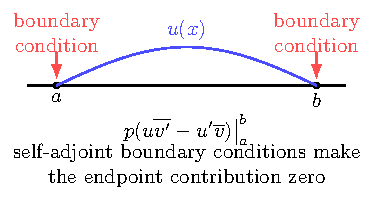
\includegraphics[width=0.56\linewidth]{figs/sturm_boundary_term.pdf}
\end{center}

\textbf{Step 3: choose boundary conditions that kill the boundary form.}  For a regular finite interval ($[a,b]$ finite, $p>0$ and $p,q,w$ finite up to both ends), standard self-adjoint boundary conditions include the
following.

\textbf{Separated real Robin conditions.}
At each endpoint impose
\begin{equation}
  \alpha_a u(a)+\beta_a(pu')(a)=0,
  \qquad
  \alpha_b u(b)+\beta_b(pu')(b)=0,
  \label{eq:robin-bc}
\end{equation}
where the coefficients are real and $(\alpha,\beta)\neq(0,0)$ at each endpoint.  The
same conditions are imposed on $v$.

To verify cancellation at one endpoint with $\beta\neq0$, substitute
$pu'=-\frac{\alpha}{\beta}u$ and $p\overline{v'}=-\frac{\alpha}{\beta}\overline v$ ($\alpha,\beta,p$ real):
\[
  \mathcal B=u(p\overline{v'})-(pu')\overline v
   =-\frac{\alpha}{\beta}u\overline v+\frac{\alpha}{\beta}u\overline v=0.
\]
The special cases $\beta=0$ ($u=v=0$, Dirichlet) and $\alpha=0$ ($pu'=pv'=0$, Neumann)
make $\mathcal B$ vanish directly.

\textbf{Periodic conditions.}
The coupled conditions
\begin{equation}
  u(a)=u(b),
  \qquad
  (pu')(a)=(pu')(b)
  \label{eq:periodic-bc}
\end{equation}
and the same for $v$ give each factor of $\mathcal B=u\,(p\overline{v'})-(pu')\,\overline v$
equal values at $a$ and $b$, so $\mathcal B(b)=\mathcal B(a)$ and the bracket in
\eqref{eq:green-identity} is zero.

\textbf{Singular endpoints.}
If $p$ vanishes at an endpoint or the interval is infinite (Legendre, $p=1-x^2$;
Hermite, $p=e^{-x^2}$; both below), no boundary condition is imposed there;
instead we keep the modes whose boundary form tends to zero:
\begin{equation}
  \lim_{x\to a^+}\mathcal B[u,v](x)=0,
  \qquad
  \lim_{x\to b^-}\mathcal B[u,v](x)=0.
  \label{eq:singular-boundary-limit}
\end{equation}
Whenever the boundary form vanishes, $(u,\ell[v])=(\ell[u],v)$: $\ell$ is symmetric,
like $D^2$ with Dirichlet ends.
\end{frame}

\begin{frame}[allowframebreaks=1.00]{The Sturm--Liouville eigenvalue problem}
\footnotesize

\textbf{The problem.} The Sturm--Liouville eigenvalue equation is
\begin{equation}
  (pu')'+qu=-\lambda wu,
  \label{eq:SLeq}
\end{equation}
with real $p,q,w$ and boundary conditions that make the boundary form \eqref{eq:SLbdy} vanish.

\textbf{Picture.} A string with tension $p(x)>0$ and mass density $w(x)>0$, held to its
rest line by springs of stiffness $-q(x)$, vibrating in a mode $u(x)\cos\omega t$,
obeys \eqref{eq:SLeq} with $\lambda=\omega^2$, which should come out real.

\textbf{Goal.} Prove that every eigenvalue $\lambda$ is real and that eigenfunctions belonging to
different eigenvalues are orthogonal with weight $w$. This repeats the matrix argument of the
previous section, with Green's identity supplying the symmetry.

\par\framebreak\par
\textbf{Step 1: insert two eigenfunctions into Green's identity.}  Let
$\ell[u_i]=-\lambda_iwu_i$ and $\ell[u_j]=-\lambda_jwu_j$.
By \eqref{eq:l2ip}, with $\overline w=w$,
\[
  (u_i,\ell[u_j])=(u_i,-\lambda_jwu_j)=-\overline{\lambda_j}\int_a^b u_i\overline{u_j}\,w\,dx=-\overline{\lambda_j}\,(u_i,u_j)_w,
\]
and likewise $(\ell[u_i],u_j)=-\lambda_i(u_i,u_j)_w$.
Green's identity \eqref{eq:green-identity} with $u=u_i$, $v=u_j$ then reads
\begin{equation}
  (\lambda_i-\overline{\lambda_j})\,(u_i,u_j)_w
  =\left[p\bigl(u_i\overline{u_j'}-u_i'\overline{u_j}\bigr)\right]_a^b .
  \label{eq:SL-lagrange-integrated}
\end{equation}
The boundary conditions make the right-hand side zero.

\textbf{Step 2: conclude, as for matrices.}  Set $j=i$: $(u_i,u_i)_w=\int_a^b w|u_i|^2\,dx>0$,
so $\lambda_i=\overline{\lambda_i}$: every eigenvalue is real.  With $\lambda_j$ real,
\eqref{eq:SL-lagrange-integrated} gives $(\lambda_i-\lambda_j)(u_i,u_j)_w=0$, hence
\begin{equation}
  (u_i,u_j)_w=0
  \qquad(\lambda_i\neq\lambda_j).
  \label{eq:SL-weighted-orthogonality}
\end{equation}
\end{frame}

\begin{frame}[allowframebreaks=0.98]{Example: Legendre equation}
\footnotesize

\textbf{Goal.} Show that the Legendre equation is a Sturm--Liouville problem, read off its
$p$, $q$, $w$, and conclude that the Legendre polynomials are orthogonal.

We take the following equation as given (Chapter~6 shows that it comes from Laplace's equation on
a sphere, with $x=\cos\theta$). For a nonnegative integer $n$, the Legendre equation is
\begin{equation}
  (1-x^2)y''-2xy'+n(n+1)y=0,
  \qquad -1<x<1.
  \label{eq:legendre-original}
\end{equation}
By the product rule, $\frac{d}{dx}\left[(1-x^2)y'\right]=(1-x^2)y''+(1-x^2)'y'=(1-x^2)y''-2xy'$,
so \eqref{eq:legendre-original} is equivalent to
\begin{equation}
  \frac{d}{dx}\left[(1-x^2)y'\right]
  =-n(n+1)y.
  \label{eq:legendre-SL}
\end{equation}
The Sturm--Liouville data are $p(x)=1-x^2$, $q(x)=0$, $w(x)=1$, $\lambda_n=n(n+1)$.

The bounded solution is the Legendre polynomial $P_n$, normalized by $P_n(1)=1$:
$P_0=1$, $P_1=x$, $P_2=\tfrac12(3x^2-1)$. Check $n=2$ in \eqref{eq:legendre-original}:
$P_2'=3x$ and $P_2''=3$, so
$(1-x^2)P_2''-2xP_2'+6P_2=3(1-x^2)-6x^2+(9x^2-3)=0$. Chapter~6 constructs the whole
family by series and Rodrigues' formula.

For $n\ne k$ the eigenvalues $n(n+1)\ne k(k+1)$, and the boundary form
$(1-x^2)(P_nP_k'-P_n'P_k)\to0$ as $x\to\pm1$, since $1-x^2\to0$ while the
polynomials and their derivatives stay finite. So \eqref{eq:SL-weighted-orthogonality} gives
orthogonality with weight $w=1$:
\begin{equation}
  \int_{-1}^{1}P_n(x)P_k(x)\,dx=0
  \qquad(n\neq k).
  \label{eq:legendre-orth}
\end{equation}
\end{frame}

\begin{frame}[allowframebreaks=1.00]{Example: Bessel equation and circular-drum modes}
\footnotesize

\textbf{Goal.} Show that the radial drum modes $J_m(\alpha s)$ solve a Sturm--Liouville problem
with weight $s$, and that modes with different $\alpha$ are orthogonal:
$\int_0^1J_m(\alpha_is)J_m(\alpha_js)\,s\,ds=0$. The only extra work, compared with Legendre, is
checking the boundary form at the drum's center $s=0$ and its rim $s=1$.

For a fixed nonnegative integer angular order $m$, the Bessel function $J_m(x)$ (the regular series solution of Chapter~3) satisfies
\begin{equation}
  x^2J_m''(x)+xJ_m'(x)+(x^2-m^2)J_m(x)=0.
  \label{eq:bessel-original}
\end{equation}
For a radial mode on the unit disk, define
\[
  y(s)=J_m(\alpha s),
  \qquad \alpha>0,
  \qquad 0\leq s\leq1.
\]
The chain rule gives $y'(s)=\alpha J_m'(\alpha s)$ and $y''(s)=\alpha^2J_m''(\alpha s)$.
Evaluate \eqref{eq:bessel-original} at $x=\alpha s$ and group each power of
$\alpha$ with its derivative:
\begin{align*}
 0&=(\alpha s)^2J_m''(\alpha s)+(\alpha s)J_m'(\alpha s)+(\alpha^2s^2-m^2)J_m(\alpha s)\\
  &=s^2\bigl[\alpha^2J_m''(\alpha s)\bigr]+s\bigl[\alpha J_m'(\alpha s)\bigr]
    +(\alpha^2s^2-m^2)J_m(\alpha s).
\end{align*}
Replacing the brackets by $y''$ and $y'$ gives
\begin{equation}
 s^2y''+sy'+(\alpha^2s^2-m^2)y=0.\label{eq:bessel-s}
\end{equation}
For $s>0$, divide by $s$ and use $(sy')'=sy''+y'$:
\[
  sy''+y'+\Bigl(\alpha^2s-\frac{m^2}{s}\Bigr)y=0
  \quad\Longleftrightarrow\quad
  (sy')'-\frac{m^2}{s}y+\alpha^2sy=0,
\]
that is,
\begin{equation}
  \frac{d}{ds}\left(s\frac{dy}{ds}\right)-\frac{m^2}{s}y
  =-\alpha^2sy.
  \label{eq:bessel-SL}
\end{equation}
Thus
\[
  p(s)=s,
  \qquad q(s)=-\frac{m^2}{s},
  \qquad w(s)=s,
  \qquad \lambda=\alpha^2.
\]
The weight $s$ is the ring-area factor: the polar area element is $s\,ds\,d\theta$,
so orthogonality over the drum's area carries a factor $s$.
Since $p(s)=s$ vanishes at $s=0$ (and $q=-m^2/s$ blows up there for $m\ge1$), $s=0$ is a
singular endpoint: we work on $[\varepsilon,1]$ and let $\varepsilon\to0^+$ at the end.

For fixed $m$, the modes $y_i(s)=J_m(\alpha_i s)$ and $y_j(s)=J_m(\alpha_j s)$ have
eigenvalues $\alpha_i^2$ and $\alpha_j^2$. Equation
\eqref{eq:SL-lagrange-integrated} on $[\varepsilon,1]$ with $p=w=s$ (everything real,
so the conjugate bars drop) gives
\begin{equation}
 (\alpha_i^2-\alpha_j^2)\int_\varepsilon^1 sy_i y_j\,ds
 =[s(y_iy_j'-y_i'y_j)]_\varepsilon^1.
 \label{eq:bessel-orth-epsilon}
\end{equation}
We must now check both endpoints; this is the part specific to the drum.

At $s=1$, impose one common boundary condition on the whole family:
\begin{itemize}
  \item Dirichlet: $y_i(1)=J_m(\alpha_i)=0$ for every $i$, so the $\alpha_i$ are the zeros
        $\alpha_{m,i}$ of $J_m$ (Chapter~3); or
  \item Neumann: $y_i'(1)=\alpha_iJ_m'(\alpha_i)=0$ for every $i$ (for $m=0$ this
        also admits $\alpha=0$: the constant mode $y=1$ with $\lambda=0$).
\end{itemize}
Either choice makes the boundary expression at $s=1$ zero.

At $s=0$, the first terms of the regular power series for $J_m$ (Chapter~3) give
\begin{align*}
  J_m(z)&=\frac1{m!}\left(\frac z2\right)^m+O(z^{m+2})
          &&(m\geq1),\\
  J_0(z)&=1-\frac{z^2}{4}+O(z^4).
\end{align*}
Hence, for $m\geq1$, $y_i=O(s^m)$ and $y_i'=O(s^{m-1})$, so
\[
  s(y_iy_j'-y_i'y_j)=O(s\cdot s^m\cdot s^{m-1})=O(s^{2m})\longrightarrow0.
\]
For $m=0$, $y_i=1+O(s^2)$ and $y_i'=O(s)$ give $O(s^2)\to0$.  (The second solutions
$Y_m$ of Chapter~3 blow up at $s=0$; they are excluded because the drum's displacement
must stay finite at the center.)

So the right side of \eqref{eq:bessel-orth-epsilon} tends to $0$ as $\varepsilon\to0^+$.
For distinct positive $\alpha_i,\alpha_j$ we have $\alpha_i^2\neq\alpha_j^2$, hence
\begin{equation}
  \int_0^1J_m(\alpha_i s)J_m(\alpha_j s)s\,ds=0
  \qquad(i\neq j).
  \label{eq:bessel-orth}
\end{equation}
\end{frame}

\begin{frame}{Legendre and Bessel modes}
\footnotesize
\begin{columns}[T,onlytextwidth]
  \begin{column}{0.49\textwidth}
    \centering
    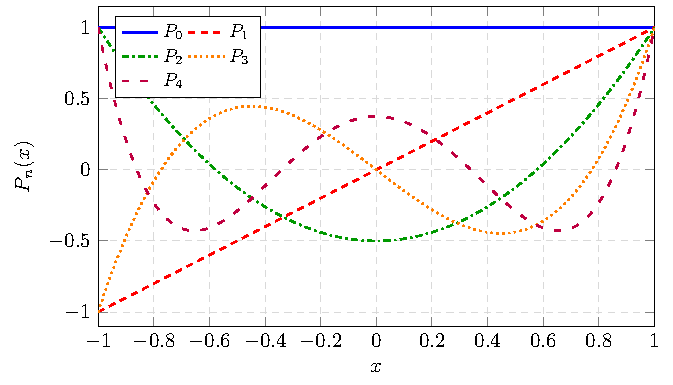
\includegraphics[width=\linewidth]{figs/legendre-P.pdf}

    \vspace{0.35em}
    Legendre modes are orthogonal on $[-1,1]$ with weight $w(x)=1$.
  \end{column}
  \begin{column}{0.49\textwidth}
    \centering
    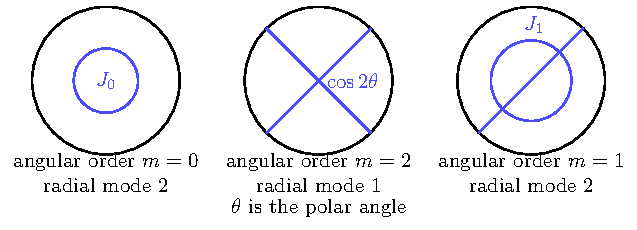
\includegraphics[width=\linewidth]{figs/bessel_disk_modes.pdf}

    \vspace{0.35em}
    Drum modes use the radial weight $w(s)=s$; a common boundary condition at
    $s=1$ selects the admissible $\alpha_i$.
  \end{column}
\end{columns}
\end{frame}

\begin{frame}[allowframebreaks=1.00]{Bringing an equation to Sturm--Liouville form}
\footnotesize

\textbf{Goal.} Rewrite a given second-order equation as $(pu')'+qu=-\lambda wu$ by an integrating
factor, so the theorem applies. Hermite first, then the general rule.

\textbf{Step 1: fully worked example---Hermite.}
Start from Hermite's equation (the quantum oscillator reduces to it, Chapter~6)
\begin{equation}
  y''-2xy'+\lambda y=0.
  \label{eq:hermite-original}
\end{equation}
Multiply it by the exponential of the integral of the $y'$ coefficient (Step~2
shows why this factor works in general):
\[
 p(x)=\exp\left(\int_0^x-2t\,dt\right)=e^{-x^2},
 \qquad p'(x)=-2xp(x).
\]
This gives $py''-2xpy'+\lambda py=0$, and the first two terms combine by the product rule,
$(py')'=py''+p'y'=py''-2xpy'$. Hence
\begin{equation}
 (e^{-x^2}y')'=-\lambda e^{-x^2}y.\label{eq:hermite-SL}
\end{equation}
The data are $p(x)=e^{-x^2}$, $q(x)=0$, $w(x)=e^{-x^2}$.
\par\framebreak\par
A polynomial solution of degree $n$ needs $\lambda_n=2n$: in \eqref{eq:hermite-original}
the $x^n$ terms are $-2nx^n$ (from $-2xy'$) and $\lambda x^n$, and must cancel.
These solutions are the physicists' Hermite polynomials $H_n$, normalized to
leading coefficient $2^n$: $H_0=1$, $H_1=2x$, $H_2=4x^2-2$.
Chapter~6 derives these by series. For example,
$H_2''-2xH_2'+4H_2=8-16x^2+16x^2-8=0$.
For $n\neq m$, $\lambda_n-\lambda_m=2(n-m)\neq0$ and the boundary form satisfies
\[
  e^{-x^2}\bigl(H_nH_m'-H_n'H_m\bigr)\longrightarrow0
  \qquad(x\to\pm\infty),
\]
because the Gaussian decays faster than any polynomial grows.  So
\eqref{eq:SL-weighted-orthogonality} with $w=e^{-x^2}$ yields
\begin{equation}
  \int_{-\infty}^{\infty}H_n(x)H_m(x)e^{-x^2}\,dx=0
  \qquad(n\neq m).
  \label{eq:hermite-orth}
\end{equation}

\textbf{Step 2: general formula.}
Now abstract the calculation.  Consider
\begin{equation}
  p_0(x)u''+p_1(x)u'+p_2(x)u=0
  \label{eq:gen2nd}
\end{equation}
with real coefficients on an interval where $p_0(x)\neq0$.  Divide by $p_0$:
\begin{equation}
  u''+\frac{p_1}{p_0}u'+\frac{p_2}{p_0}u=0.
  \label{eq:gen2nd-div}
\end{equation}
Define the integrating factor
\begin{equation}
  p(x)=\exp\left(\int_{x_0}^{x}\frac{p_1(t)}{p_0(t)}\,dt\right).
  \label{eq:intfactor}
\end{equation}
The chain rule gives $p'=(p_1/p_0)p$. This is the integrating-factor trick for
$y'+Py=f$: $p$ is chosen so that the two derivative terms collapse into one exact
derivative. Multiplying \eqref{eq:gen2nd-div} by $p$ gives
$pu''+p'u'+p\frac{p_2}{p_0}u=0$, and $pu''+p'u'=(pu')'$, so
\begin{equation}
 (pu')'+qu=0,
 \qquad q=p\,\frac{p_2}{p_0}.
 \label{eq:gen2nd-SL}
\end{equation}
Equivalently, without first dividing by $p_0$, multiply the original equation
\eqref{eq:gen2nd} by $p/p_0$ (not by $p$ alone).

\par\framebreak\par
If the spectral parameter occurs as
\begin{equation}
  p_0u''+p_1u'+\bigl(r_0(x)+\lambda r_1(x)\bigr)u=0,
  \label{eq:gen-spectral}
\end{equation}
multiplying by $p/p_0$ exactly as for \eqref{eq:gen2nd-SL} gives
$(pu')'+p\frac{r_0}{p_0}u+\lambda p\frac{r_1}{p_0}u=0$; moving the $\lambda$ term
to the right,
\begin{equation}
  (pu')'+qu=-\lambda wu,
  \qquad
  q=p\frac{r_0}{p_0},
  \qquad
  w=p\frac{r_1}{p_0}.
  \label{eq:gen-spectral-SL}
\end{equation}
The theory above needs $w>0$: if $r_1/p_0<0$ on the interval, replace $\lambda$
by $-\lambda$ and $w$ by $-w$.
\end{frame}

% ======================================================================
\section{Green's function on an interval}
% ======================================================================

\begin{frame}[allowframebreaks=1.00]{A unit point source creates a jump}
\footnotesize
\textbf{Goal.} Solve the \emph{forced} problem \(Lu=f\) (for example a string under a distributed load
\(f\)) for every \(f\) at once.

\textbf{Plan.} First find the response to a load concentrated at a single point \(x'\). A general load
is a sum of such point loads, so the general response is the sum (integral) of point responses.

\textbf{Setting.} On a finite interval \([a,b]\) take
\[
 L[u]=-(pu')'-qu=-\ell[u]
\]
(\(\ell\) from \eqref{eq:SLop}; the minus sign makes \eqref{eq:SLeq} read \(Lu=\lambda wu\)), with the boundary conditions
\eqref{eq:robin-bc}.

\textbf{A unit point load: the Dirac delta \(\delta(x-x')\).} Think of it as a very tall, very narrow spike
at \(x'\) with total area \(1\). Its defining property: for continuous \(f\) and \(a<x'<b\),
\[
 \int_a^b\delta(x-x')f(x)\,dx=f(x'),
\]
and likewise \(\int_a^b\delta(x-x')f(x')\,dx'=f(x)\). The \emph{Green function} \(G(x,x')\) is the response to a
unit load at \(x'\): it solves \(L_xG=\delta(x-x')\) (\(L\) acting on the variable \(x\)) with the boundary
conditions.
\par\framebreak\par
\begin{columns}[T]
\begin{column}{0.55\textwidth}
\footnotesize
\textbf{First by hand: a fixed string.} Take \(p=1\), \(q=0\) on \([0,1]\): \(-G''=\delta(x-x')\), with
\(G(0)=G(1)=0\).

\emph{Away from \(x'\)}, \(G''=0\), so \(G\) is a straight line on each side. The lines must pass through the
fixed ends:
\[
 G=c_1x\ (x<x'),\qquad G=c_2(1-x)\ (x>x').
\]
\emph{At \(x'\)}, two physical conditions:
\begin{itemize}
 \item the string does not break (continuity): \(c_1x'=c_2(1-x')\);
 \item force balance: the unit load equals the tension (\(=1\)) times the drop in slope. The slope
       changes from \(c_1\) to \(-c_2\): \(\;-c_2-c_1=-1\), so \(c_1+c_2=1\).
\end{itemize}
\end{column}
\begin{column}{0.43\textwidth}
\centering
\begin{tikzpicture}[x=3.3cm,y=6cm]
 \draw[->] (0,0) -- (1.1,0) node[right] {$x$};
 \draw[->] (0,0) -- (0,0.31) node[above] {$G$};
 \draw (1,0.01) -- (1,-0.01) node[below] {$1$};
 \draw[dashed,gray] (0.7,0) -- (0.7,0.21);
 \node[below] at (0.7,0) {$x'$};
 \draw[blue!70!black,thick] (0,0) -- node[sloped,above,inner sep=1pt] {slope $1-x'$} (0.7,0.21) -- (1,0);
 \draw[->,red!75!black,thick] (0.7,0.215) -- (0.7,0.29) node[right] {unit load};
 \node[blue!70!black,anchor=west] at (0.9,0.1) {slope $-x'$};
\end{tikzpicture}
\end{column}
\end{columns}
\par\framebreak\par
\emph{Solve.} Put \(c_2=1-c_1\) into the continuity condition:
\(c_1x'=(1-c_1)(1-x')=1-x'-c_1+c_1x'\), so \(c_1=1-x'\) and then \(c_2=x'\). With \(x_<=\min(x,x')\),
\(x_>=\max(x,x')\),
\[
 G(x,x')=x_<\,(1-x_>):
\]
a tent with its peak at the load.


\textbf{The general case: the same two facts.}

\emph{Step 1: away from \(x'\).} There \(L_xG=0\). Let \(y_L\) be a solution of \(Ly=0\) that satisfies the
\emph{left} boundary condition, and \(y_R\) one that satisfies the \emph{right} one. Then
\[
 G=c_1\,y_L(x)\ (x<x'),\qquad G=c_2\,y_R(x)\ (x>x').
\]
(We assume \(0\) is not an eigenvalue, that is, \(Lu=0\) with both boundary conditions only has
\(u=0\). Then \(y_L\) and \(y_R\) are not multiples of each other, so their Wronskian
\(W[y_L,y_R]=y_Ly_R'-y_L'y_R\) is not zero. A string with both ends free fails this: \(u=\)const solves
\(Lu=0\), and nothing holds the string against a point load.)

\emph{Step 2: the slope jumps (force balance).} Integrate \(-(pG')'-qG=\delta(x-x')\) over a tiny interval
\([x'-\varepsilon,x'+\varepsilon]\). The \(\delta\) integrates to \(1\):
\[
 -\bigl[pG'\bigr]_{x'-\varepsilon}^{x'+\varepsilon}
 -\int_{x'-\varepsilon}^{x'+\varepsilon}qG\,dx=1 .
\]
As \(\varepsilon\to0\), the \(qG\) integral vanishes (a bounded function over a shrinking interval), and the
bracket becomes \(p(x')\bigl[G'(x'^+)-G'(x'^-)\bigr]\). So
\begin{equation}
 G'(x'^+,x')-G'(x'^-,x')=-\frac1{p(x')} .
 \label{eq:green-jump}
\end{equation}
The slope drops by (load)/(tension), as for the string.


\emph{Step 3: \(G\) is continuous (the string does not break).} \(G'\) only jumps by a finite amount, so it
stays bounded, and the change of \(G\) across the tiny interval,
\(\int_{x'-\varepsilon}^{x'+\varepsilon}G'\,dx\), tends to \(0\). So \(c_1y_L(x')=c_2y_R(x')\). A symmetric way to satisfy this is
\(c_1=A\,y_R(x')\), \(c_2=A\,y_L(x')\) for some constant \(A\):
\[
 G(x,x')=
 \begin{cases}
  A\,y_L(x)\,y_R(x'), & x<x',\\[2pt]
  A\,y_L(x')\,y_R(x), & x>x'.
 \end{cases}
\]
\emph{Step 4: find \(A\) from the jump.} Differentiate each branch in \(x\) and set \(x=x'\):
\(G'(x'^+)=A\,y_L(x')\,y_R'(x')\) and \(G'(x'^-)=A\,y_L'(x')\,y_R(x')\). Their difference is
\(A\bigl[y_Ly_R'-y_L'y_R\bigr](x')=A\,W(x')\). By \eqref{eq:green-jump},
\[
 A\,W[y_L,y_R](x')=-\frac1{p(x')},\qquad A=-\frac{1}{p(x')\,W(x')}.
\]


\emph{Step 5: \(A\) does not depend on \(x'\).} Divide \(Ly=0\) by \(-p\): \(y''+\frac{p'}{p}y'+\frac qp\,y=0\). By Abel's
identity (Chapter~3), \(W=C\exp\bigl(-\int\frac{p'}{p}dx\bigr)=C\,e^{-\log p}=\frac{C}{p}\). So \(p\,W=C\) is a
constant, and so is \(A=-1/C\).

\textbf{Result.} With \(x_<=\min(x,x')\), \(x_>=\max(x,x')\),
\begin{equation}
 G(x,x')=-\frac{y_L(x_<)\,y_R(x_>)}{p\,W[y_L,y_R]}.
 \label{eq:green-two-sol}
\end{equation}
\emph{Check (string):} \(y_L=x\), \(y_R=1-x\), \(p=1\), and \(W=x\cdot(-1)-1\cdot(1-x)=-1\). So
\(G=-\frac{x_<(1-x_>)}{-1}=x_<(1-x_>)\), the tent.

\textbf{Superposition.} A load \(f\) is a sum of point loads \(f(x')\,dx'\). So the response is
\(u(x)=\int_a^bG(x,x')f(x')\,dx'\). Check: \(L\) acts on \(x\) only, so
\[
 L_xu=\int_a^b L_xG(x,x')\,f(x')\,dx'=\int_a^b\delta(x-x')\,f(x')\,dx'=f(x),
\]
and \(u\) satisfies the boundary conditions because each \(G(\cdot,x')\) does.
\end{frame}

\begin{frame}[allowframebreaks=1.00]{The same function written in eigenfunctions}
\footnotesize
\textbf{Why a second form.} Formula \eqref{eq:green-two-sol} is closed but hides the
modes. Expanding $G$ in the eigenfunctions of $L$ shows how strongly each mode
answers the load.

Let $L\phi_n=\lambda_nw\phi_n$ with real eigenfunctions, assumed complete, and weighted
norm $N_n=\int_a^bw\phi_n^2\,dx$; $\lambda_n\ne0$ because $0$ is not an eigenvalue.
Write $G(x,x')=\sum_nc_n\phi_n(x)$ and apply $L_x$ term by term:
\[
 \delta(x-x')=L_xG=\sum_{n}c_n\lambda_n\,w(x)\phi_n(x).
\]
Multiplying by $\phi_m(x)$ and integrating over $[a,b]$,
\[
 \phi_m(x')=\int_a^b\delta(x-x')\phi_m(x)\,dx
 =\sum_nc_n\lambda_n\int_a^bw\phi_n\phi_m\,dx
 =c_m\lambda_mN_m,
\]
by the delta's defining property, then weighted orthogonality
\eqref{eq:SL-weighted-orthogonality} (only $n=m$ survives). Hence
$c_m=\phi_m(x')/(\lambda_mN_m)$ and
\begin{equation}
 G(x,x')=\sum_{n=1}^{\infty}\frac{\phi_n(x)\,\phi_n(x')}{\lambda_nN_n}.
 \label{eq:green-spectral}
\end{equation}
\textbf{Meaning.} Mode $n$ is excited in proportion to $\phi_n(x')$ (a load at a node
of $\phi_n$ does not excite it) and weakened by $1/\lambda_n$: stiff, high-frequency
modes respond little.

\textbf{Example (fixed string).} Here $\phi_n=\sin(n\pi x)$ and $\lambda_n=(n\pi)^2$
(\eqref{eq:string-eigenpairs} with the sign of $L$ flipped), and $N_n=1/2$ by \eqref{eq:sin-nn}.
The tent of the previous frame is therefore
\[
 x_<(1-x_>)=\sum_{n=1}^{\infty}\frac{2\sin(n\pi x)\sin(n\pi x')}{(n\pi)^2};
\]
at $x=0.3$, $x'=0.7$ both sides equal $0.3\cdot0.3=0.09$.

\textbf{Completeness relation.} Expand any $f(x)=\sum_nb_n\phi_n(x)$. The projection
formula \eqref{eq:coeff-orthogonal} in the weighted inner product \eqref{eq:wip} gives
$b_n=\frac1{N_n}\int_a^bw(x')\phi_n(x')f(x')\,dx'$; substituting and exchanging sum and
integral,
\[
 f(x)=\int_a^b\Bigl[\sum_n\frac{\phi_n(x)\phi_n(x')}{N_n}\Bigr]w(x')f(x')\,dx'.
\]
Since also $f(x)=\int_a^b\delta(x-x')f(x')\,dx'$ for every $f$, the bracket times
$w(x')$ acts as $\delta(x-x')$:
\begin{equation}
 \sum_{n=1}^{\infty}\frac{\phi_n(x)\,\phi_n(x')}{N_n}
 =\frac{\delta(x-x')}{w(x')}.
 \label{eq:completeness}
\end{equation}

\begin{columns}[T]
\begin{column}{0.5\textwidth}
\footnotesize
\textbf{Meaning.} Added together, the modes rebuild a sharp spike at $x'$, so they can
build any source. For the string ($w=1$, $N_n=1/2$) the partial sums
$\sum_{n=1}^N2\sin(n\pi x)\sin(n\pi x')$ at $x'=\tfrac12$ grow a peak of height about
$N$ and width about $1/N$ at $x'$, with area near $1$: they approach a delta.
\end{column}
\begin{column}{0.48\textwidth}
\centering
\begin{tikzpicture}[x=4.4cm,y=0.1cm]
 \draw[->] (0,0) -- (1.08,0) node[right] {$x$};
 \draw[->] (0,-5) -- (0,23);
 \foreach \t in {10,20} \draw (0.01,\t) -- (-0.01,\t) node[left] {$\t$};
 \draw (1,0.6) -- (1,-0.6) node[below] {$1$};
 \draw[blue!70!black] plot[domain=0:1,samples=200]
   (\x,{sin(5.5*180*(\x-0.5))/(2*sin(90*(\x-0.5)))-sin(5.5*180*(\x+0.5))/(2*sin(90*(\x+0.5)))});
 \draw[red!75!black] plot[domain=0:1,samples=200]
   (\x,{sin(20.5*180*(\x-0.5))/(2*sin(90*(\x-0.5)))-sin(20.5*180*(\x+0.5))/(2*sin(90*(\x+0.5)))});
 \node[blue!70!black,anchor=west] at (0.58,7) {$N=5$};
 \node[red!75!black,anchor=west] at (0.56,18) {$N=20$};
\end{tikzpicture}
\end{column}
\end{columns}
\end{frame}

\begin{frame}[allowframebreaks=0.98]{Chapter summary}
\footnotesize

\begin{itemize}
 \item Functions behave as vectors under $(u,v)=\int_a^b u\overline v\,dx$,
 or its weighted version. Our convention is linear in the first slot:
 $(cu,v)=c(u,v)$, $(u,cv)=\overline c(u,v)$.
 \item Orthogonality gives coefficients by projection:
 $a_n=(f,u_n)/\|u_n\|^2$. For $u_n=\sin(n\pi x)$ on $(0,1)$,
 $\|u_n\|^2=1/2$.
 \item Integration by parts identifies both the formal adjoint and the boundary
 term. The expression $p_0u''+p_1u'+p_2u$ with real coefficients is formally
 self-adjoint when $p_1=p_0'$, giving $(pu')'+qu$.
 \item Boundary conditions must make
 $[p(u\overline{v'}-u'\overline v)]_a^b$ vanish. Under these conditions and
 a positive weight, $(pu')'+qu=-\lambda wu$ has real eigenvalues and
 weighted-orthogonal eigenfunctions for distinct eigenvalues.
 \item Multiplying a general second-order equation by an integrating factor
 puts its derivative terms into $(pu')'$, with
 $p=\exp\int(p_1/p_0)\,dx$. The Legendre, Bessel, and Hermite weights are
 $1$, $s$, and $e^{-x^2}$.
 \item For $L=-(pu')'-qu$, the Green function, the response to a unit point load,
 solves $LG=\delta(x-x')$: it is continuous at $x'$, its derivative jumps by
 $-1/p(x')$ (a tent $x_<(1-x_>)$ for the fixed string), and it can be written
 either as $-y_L(x_<)y_R(x_>)/(pW)$ \eqref{eq:green-two-sol} or as the modal
 series \eqref{eq:green-spectral}; the basis also satisfies the completeness
 relation \eqref{eq:completeness}.
\end{itemize}
\end{frame}

\end{document}
